\chapter{Foundations}
\label{ch:foundations}

For the development of this work, some foundations about thermal modeling and model predictive control (MPC) are needed, which are explained in this chapter. Note, that in the following all vectors are in thick print, like \textbf{x}.

\section{Thermal basics}
\label{section:thermalbasics}

There are three different mechanism, which describe physically the heat transfer: Heat conduction, heat convection and heat irradiation\cite{.2013}. Every mechanism is used for thermal modelling of buildings. For example, conduction is the main part of heat transfer through walls or floors. Convection takes place inside and outside between the walls and the air and irradiation is needed for the integration of the impact of the sun, for example.

\subsection{Conduction}
\label{subsection:conduction}

    Conduction means, that heat energy is directed in a solid or fluid. Molecules within the solid or fluid have higher energy when the temperature is higher. They transfer the energy to neighbour molecules with smaller energy. Without a heat source, the temperature difference between the a hot and a cold location of the molecules decrease.\cite{Kuchling.2007}
    \newline The equation \ref{eq:fourier} describes the conduction according to Fourier \cite{.2013}. There is $\lambda$ the thermal conductivity with the assumption of being constant and $\dot{\textbf{q}}$ and $T$ represent the specific heat flux and the temperature. The thermal conductivity is dependent on the material, such as concrete, wood or bricks. 
    \begin{equation}
    \label{eq:fourier}
        \dot{\textbf{q}} = - \lambda grad T
    \end{equation}
    For the further work, it will be relevant to expand the above equation with the area $A$, the thickness of the conductive medium $d$ and an temperature difference $\Delta T$ assuming one significant direction of the heat flux $\dot{Q}$ to:
    \begin{equation}
    \label{eq:conduction}
        \dot{Q} = \frac{A\lambda}{d} \Delta T
    \end{equation}
    In therms of buildings, the conductive medium could be walls, floors or roofs.
    \newline
    Further, the Ohm's law of thermodynamics describes the above equation as 
     \begin{equation}
    \label{eq:conduction}
        \dot{Q} = \frac{\Delta T}{R_\lambda} 
    \end{equation}
    and determine the thermal resistance $R_\lambda$ as
    \cite{Kuchling.2007}
    \begin{equation}
    \label{eq:r_lambda}
        R_\lambda = \frac{d}{A\lambda}
    \end{equation}
    what is required for the RC- modeling of buildings, which is nearly explained in \ref{section:modeling}.

\subsection{Convection}
\label{subsection:convection}

    Macroscopic movements of a fluid  lead to transport of kinetic energy and enthalpy, called convection. These movements are generated by external forces or by internal forces like balancing the pressure or temperature.\cite{.2013}
    \newline
    Newton's law of cooling describes the heat transfer of convection $\dot{Q}$ as 
    \begin{equation}
    \label{eq:newton}
        \dot{Q} = \alpha A (T_w - T_\infty)
    \end{equation}
    with the heat transfer coefficient $\alpha$, especially for building modeling the wall temperature $T_w$ and the environment temperature $T_\infty$ \cite{Griesinger.2019}
    . There are two possibilities to determine the heat transfer coefficient. Both require a temperature difference $\Delta T$ and either a temperature gradient $\partial T/\partial x$ or a heat flux $\dot{Q}$.
    \cite{.2013} 
    \newline
    The conversion of the equation \ref{eq:newton} leads to the thermal resistance for convection, shown in the next equation.\cite{Griesinger.2019}
    \begin{equation}
        R_\alpha = \frac{\Delta T}{\dot{Q}} = \frac{1}{\alpha A}
    \end{equation}

\subsection{Radiation}
\label{subsection:radiation}

    Every body emits heat radiation at the environment with electromagnetic waves. As shown in the following equation, the temperature $T$ of the body influences highly the heat radiation.\cite{.2013} 
    \begin{equation}
    \label{eq:radiation}
        \dot{q} = \sigma T^4
    \end{equation}
    This correlation applies to a black body, where $\dot{q}$ is a heat flux and $\sigma$ represents the Stefan- Boltzmann coefficient. A black body absorbs all heat radiation with all wave length of all directions\cite{Griesinger.2019}. The consideration of a black body is idealized, for the illustration of a real body (see equation \ref{eq:realbodyradiation}) the emissivity $\epsilon$ is used. $\epsilon$ is material-dependent and lies between 0 and 1.
    \begin{equation}
    \label{eq:realbodyradiation}
        \dot{q} = \epsilon \sigma T^4
    \end{equation}
    Especially, heat radiation only does not need matter for energy transportation.\cite{.2013}
    \newline
    The best known source of heat radiation is the sun, which plays an important roll in thermal modeling of buildings. Objectives in the building, such as radiators, also  radiate heat. For example, Radiators have equal parts convective and radiative energy transport \cite{Hazyuk.2012}. 
  %hier noch näher auf Absorbtion, Transsmission und REflexion eingehen, wird reflexion vllt bei fenstern gebraucht, absorbtion beim Aufheizen von boden oder ähnlichem  
    
    
\section{Lumped capacitance model}
\label{section:modeling}
For modeling the thermal behavior of buildings, the lumped capacitance model is often used. With this approach, using the electrical analogy, building elements can be easily represented by resistors $R$ and capacitors $C$. \cite{Kramer.2012}

\subsection{Electrical analogy}
\label{electricalanalogy}

    Similar to an electrical network, the potential is represented by the temperature at one node, the heat flux corresponds to the current and thermal resistances $R$ comply with electrical resistors and thermal capacitance $C$ with electrical capacitors. The thermal capacitance is the specific heat capacity $c$ multiplied by the mass $m$ ($C=cm$). All connections in a network have impact on each other. For a better explanation, a simple exampling thermal network is mapped in the next figure, which represents a heated wall of a building.
    \begin{figure}[h]
    \centering
    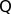
\includegraphics[scale=0.8]{figure/beispiel Netzwerk.png}
    \caption{Sample RC- network}
    \label{fig:sampleRCnetwork}
    \end{figure}
    The heat flux $\dot{Q}$, for example from an radiator, influence the temperature $T_wall$, as well as the capacity $C$, the temperature inside and outside $T_inside$ and $T_outside$ with their resistances $R_\alpha,inside$ and $R_\alpha,outside$.
    For creating the differential equation, the Kirchhoff's Current Law is required. It states that the sum of the flowing current to the node is equal to the sum of the flowing current off the node 
    \cite{Kuchling.2007}. 
    Since there is a thermal modeling case, the current is replaced by the heat flux. The following differential equation results for the node  $T_{wall}$ using the Ohm's law ($\dot{Q}=\Delta T/R$) and the relationship $\dot{Q}=C\frac{\partial T}{\partial t}$.     
    \begin{equation}
    \label{eq:sampledifferential}
    C \frac{\partial T_{wall}}{\partial t} = \dot{Q} + \frac{T_{inside}-T{wall}}{R_\alpha,inside} - \frac{T_{wall}-T{outside}}{R_\alpha,outside}
    \end{equation}
    In the shown figure, the thermal resistances are serial connected. According to the electrical network, the summary resistance is the sum of these two resistance. 
    \begin{equation}
    \label{eq:resistanceseriel}
        R_{sum} = R_{\alpha,inside} + R_{\alpha,outside}
    \end{equation}
    A parallel circuitry has windows and walls in buildings, for example. Here the resistances are calculated according to the following schema:
    \begin{equation}
    \label{eq:resistancesparallel}
        \frac{1}{R_{sum}} = \frac{1}{R_{wall}} + \frac{1}{R_{window}}
    \end{equation}
    In terms of needed more capacities for describing the thermal model, the summary capacity are added in a parallel circuitry as: 
    \begin{equation}
    \label{eq:capacity}
         C_{sum} = C_1 + C_2
    \end{equation}
    The serial circuitry of capacities will not used in this work, thus it is not nealy explained.
%maschenregel noch erklären?
\section{Model predictive control (MPC)}
\label{section:mpc}
"The idea of model predictive control [...] is [..] to utilize a model of the process in order to predict and optimize the future system behavior."
\cite{Grune.2017}
Applied to a thermal control of a building with the aim of grid- supporting, a model of the thermal behavior of the building is required to predict the reaction of the system behavior in the next $N$ time steps, called the prediction horizon. Every time step $k$, the current state \textbf{$x_k$}, the output \textbf{$y_k$} and the future system behavior is obtained via measurements and computation. The computation of the future system behavior includes water forecast, occupant schedule  and the optimization of the control signal \textbf{$u_k$} over the optimization horizon \textbf{$u_{k+N}$}. But, only the first calculated control signal is adopt as input for the plant.
Then, the proceeding repeat every time step the calculations. 
 \begin{figure}[h]
    \centering
    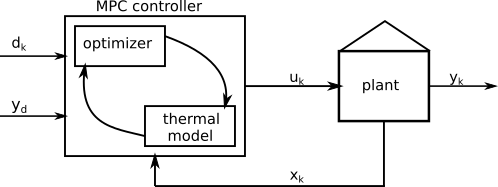
\includegraphics[scale=0.8]{figure/MPC beispiel2.png}
    \caption{MPC structure of the control loop}
    \label{fig:sampleMPC}
    \end{figure}
\newline
Concluded, the MPC is "an iterative online optimization over the predictions"
\cite{Grune.2017} 
compiled by the thermal model of the building. Mathematically explained, the optimizer needs to reduce the following equation according to
\cite{Kouvaritakis.2018}
and
\cite{Oldewurtel.2012}:
\begin{align}
\label{eq:costfunc}
\textrm{Cost function} && minimize \sum_{k=1}^{N-1} c_k(x_k,u_k,y_k)
\end{align}
subject to 
\begin{align*}
\textrm{Current state} && x_0 &=& x \\	
\textrm{Dynamics} && x_{k+1}&=& f(x_k,u_k,d_k)		&&	y_k = g(x_k,u_k,d_k)\\				
\textrm{Constraints} && y_{min}&\leq& y_k \leq y_{max}\\		
\textrm{} && u_{min}&\leq& u_k \leq u_{max}	
\end{align*}
$c_k$ represents the cost function, which is nearly explained in the next subsection  \ref{subsection:costfunction}
. In therms of building control, $y$ is the internal temperature.
%Störungen noch erklären
\subsection{Cost function}
\label{subsection:costfunction}
The cost function $c_k$ optimize the control signal $u_k$ for the current state $x_k$, which is mathematically described in equation
\ref{eq:costfunc}
, with:
\begin{equation}
\label{eq:c_k}
c_k = (x_k^TQx_k+u_k^TRu_k)
\end{equation}
Here $Q$ and $R$ are matrices over which individual elements of the state vector or control signal vector can be weighted differently.  
\cite{Kouvaritakis.2016}
%linear, quadratisch, gewichtet 
%reduziert Zustand, stellsignal
\subsection{Current state}
\label{subsection:currentstate}
The current state $x_k$ is a vector of measured state variables of a building. Every prediction starts form this initial state\cite{Oldewurtel.2012}.
\subsection{Dynamics}
\label{subsection:dynamics}
\begin{align}
\label{eq:statespace}
\dot{x}=Ax+B_1u+B_2d\\
y=Cx+D_1u+D_2d
\end{align}


\subsection{Constraints}
\label{subsection:constraints}



%Abbildung zu Regelsstrecke erstellen. Eingänge/Ausgänge, Modell, Optimierer usw

%This chapter is supposed to summarize previous work of other researchers related to your topic.
%The aim is to give an overview of existing literature while highlighting differences and similarities to this thesis.
%
%Please choose a coherent citation style throughout the thesis. For example
%
%\begin{itemize}
%	\item Direct citation of results, an approach or similar
%	\item[] \Textcite{Fan.2015} find that their method improves the benchmark.
%	\item Indirect citation
%	\item[] Recent research highlights the importance of this method \Parencite{Fan.2015}.
%	\item Direct citation
%	\item[] \textquote{\emph{Energy optimisation in buildings is important}} \Parencite{Fan.2015}.
%\end{itemize}



